%!TEX TS-program = xelatex
%!TEX encoding = UTF-8 Unicode

\def \papersize {a4paper}
\documentclass[12pt,\papersize]{extarticle}
% extarticle is like article but can handle 8pt, 9pt, 10pt, 11pt, 12pt, 14pt, 17pt, and 20pt text

\def \ititle {How to Construct a Minimal Theory of Mind}
\def \isubtitle {}
\def \iauthor {Stephen A. Butterfill \& Ian A. Apperly}
\def \iemail{s.butterfill@warwick.ac.uk}
%for anonymous submisison
%\def \iauthor {}
%\def \iemail{}
%\date{}

%!TEX TS-program = xelatex
%!TEX encoding = UTF-8 Unicode

\title{\ititle\\\isubtitle}
\author{\iauthor\\<{\iemail}>}

\usepackage[\papersize]{geometry} % see geometry.pdf
\geometry{twoside=false}
\geometry{headsep=2em} %keep running header away from text
\geometry{footskip=1cm} %keep page numbers away from text
\geometry{top=3cm} %increase to 3.5 if use header
\geometry{left=4cm} %increase to 3.5 if use header
\geometry{right=4cm} %increase to 3.5 if use header
\geometry{textheight=22cm}

%non-xelatex
%\usepackage[T1]{fontenc}
%\usepackage{tgpagella}

%for underline
\usepackage[normalem]{ulem}

%get the font here:
% http://scripts.sil.org/CharisSILfont

\usepackage{fontspec,xunicode}
%nb do not explicitly use package xltxtra because this introduces bugs with footnote superscripting  -- perhaps because fontspec is supposed to include it anyway.
%UPDATE:  "You need to use the no-sscript option in xltxtra: \usepackage[no-sscript]{xltxtra}, this is explained in the documentation of xltxtra.  The issue is that Sabon does not contain true superscript glyphs for every character and the no-sscript option will instead use scaled regular glyphs, which is typographically inferior, but there is no other option available when using Sabon." --- http://groups.google.com/group/comp.text.tex/browse_thread/thread/19de95be2daacade
\defaultfontfeatures{Mapping=tex-text}
%\setromanfont[Mapping=tex-text]{Charis SIL} %i.e. palatino
%\setromanfont[Mapping=tex-text]{Sabon LT Std} 
%\setromanfont[Mapping=tex-text]{Dante MT Std} 
%\setromanfont[Mapping=tex-text,Ligatures={Common}]{Hoefler Text} %comes with osx
\setromanfont[Mapping=tex-text]{Linux Libertine O} 
\setsansfont[Mapping=tex-text]{Linux Biolinum O} 
\setmonofont[Scale=MatchLowercase]{Andale Mono}


%hyperlinks and pdf metadata
%TODO avoid duplication of title & author
\usepackage{hyperref}
\hypersetup{pdfborder={0 0 0}}
\hypersetup{pdfauthor={\iauthor}}
\hypersetup{pdftitle={\ititle\isubtitle}}


%handles references to labels (e.g. sections) nicely
\usepackage{varioref}

%line spacing
\usepackage{setspace}
%\onehalfspacing
%\doublespacing
\singlespacing

\usepackage{natbib}
%\usepackage[longnamesfirst]{natbib}
\setcitestyle{aysep={}}  %philosophy style: no comma between author & year

%enable notes in right margin, defaults to ugly orange boxes TODO fix
%\usepackage[textwidth=5cm]{todonotes}

%for comments
\usepackage{verbatim}

%footnotes
\usepackage[hang]{footmisc}
\setlength{\footnotemargin}{1em}
\setlength{\footnotesep}{1em}
\footnotesep 2em

%tables
\usepackage{booktabs}
\usepackage{ctable}

%section headings
\usepackage[sf]{titlesec}
%\titlespacing*{\section}{0pt}{*3}{*0.5} %reduce vertical space after header
%large headings:
%\titleformat{\section}{\LARGE\sffamily}{\thesection.}{1em}{} 
\titlelabel{\thetitle.\quad}

%captions
\usepackage[font={small,sf}, margin=0.75cm]{caption}

%lists
\usepackage{enumitem}
\newenvironment{idescription}
{ 	
	% begin code
	\begin{description}[
		labelindent=1.5\parindent,
		leftmargin=2.5\parindent
	]
}
{ 
	%end code
	\end{description}
}


%title
\usepackage{titling}
\pretitle{
	\begin{center}
	\sffamily
	\Huge
} 
\posttitle{
	\par
	\end{center}
	\vskip 0.5em
} 
\preauthor{
	\begin{center}
	\normalsize
	\lineskip 0.5em
	\begin{tabular}[t]{c}
} 
\postauthor{
	\end{tabular}
	\par
	\end{center}
}
\predate{
	\begin{center}
	\normalsize
} 
\postdate{
	\par
	\end{center}
}



\begin{document}

\setlength\footnotesep{1em}

\bibliographystyle{newapa} %apalike

%these two lines are for anonymous submission --- they remove author and date
%but don't forget to remove defs above as well --- otherwise it will be in the metadata
%\author{}
%\date{}


\maketitle
%\tableofcontents

\begin{abstract}
\noindent
What could someone represent that would enable her to track, at least within limits, perceptions, beliefs including false beliefs, and other propositional attitudes? 
An obvious possibility is that she might represent these very propositional attitudes as such.
It is sometimes tacitly or explicitly assumed that this is the only possible answer.
However we argue that several recent discoveries in developmental, cognitive, and comparative psychology indicate the need for other, less obvious possibilities.
Our aim is to meet this need by describing the construction of a minimal theory of mind.  
Minimal theory of mind is rich enough to explain systematic success on tasks held to be acid tests for theory of mind cognition including many false belief tasks.  
It is also extensible in ways that can explain a wide range of findings from non-human animals and human infants that are sometimes presented as evidence for full-blown theory of mind cognition.  
Yet minimal theory of mind does not require representing propositional attitudes, or any other kind of representation, as such.
Minimal theory of mind may be what enables those with limited cognitive resources or little conceptual sophistication, such as infants, chimpanzees, scrub-jays and human adults under load, able to track, within limits, facts about perceptions and beliefs.

\ 

\noindent
\textbf{Keywords:}
Theory of Mind, False Belief, belief, perception, development, comparative
\end{abstract}



\section{Introduction}
What could someone represent that would enable her to track, at least within limits, perceptions, beliefs including false beliefs, and other propositional attitudes? 
One answer is obvious: she might track these things by virtue of representing them as such, that is, by representing perceptions, beliefs, and other propositional attitudes as such.
Our aim in what follows is to identify another, less obvious answer.
There is a form of cognition---minimal theory of mind---which does not involve representing propositional attitudes as such but does involve representing simpler, relational mental states which could, within limits, enable one to track propositional attitudes such as beliefs.
Minimal theory of mind 
is  rich enough to enable systematic success on tasks held to be acid tests for theory of mind cognition including many false belief tasks.
As we will explain, this has consequences 
for interpreting a range of findings concerning infants', adults' and nonhumans' performances on theory of mind tasks.
It may help us to understand what enables those with limited cognitive resources or little conceptual sophistication, such as infants, chimpanzees, scrub-jays and human adults under load, to track, within limits, facts about perceptions and beliefs.

In this section we defend explain our question; in the next sections we introduce the findings which motivate facing it before starting to answer it in the fourth section.

Some may find our question initially incomprehensible.
Could abilities to track false beliefs (say) really involve anything other than representing false beliefs?
To see the possibility of a positive answer it may help to consider a non-mental analogy.
What could someone represent that would enable her to track, at least within limits, the toxicity of potential food items?
Here the most straightforward answer (she could represent their toxicity) is clearly not the only one.
After all, someone might track toxicity by representing odours or by representing visual features associated with putrefaction, say.
Suppose Sin\'ead has no conception of toxins but represents the odours of food items and 
treats those with foul odours as dangerous to eat,
so that she would not normally offer them to friends or family
nor conceal them from competitors.
This brings nutritional and competitive benefits obtaining which depends on facts about toxicity.
If Sin\'ead tends to behave in this way because of these benefits, 
representing odours enables her to track, in a limited but useful range of cases,  toxicity.
Our question, put very roughly, is whether   belief has something like an odour.

To make the question more precise it is useful to distinguish 
theory of mind abilities from theory of mind cognition.  
A  \textit{theory of mind ability} is an ability that exists in part because exercising it brings benefits obtaining which depends on exploiting or influencing facts about others’ mental states.
To illustrate,
suppose that Hannah is able to discern whether another's eyes are in view,
that Hannah exercises this ability to escape detection while stealing from others,
that Hannah's ability exists in part because it benefits her in this way,
and 
that Hannah's escaping detection depends on exploiting a fact about other's mental states (namely that they usually cannot  see Hannah's acts of theft when Hannah doesn't have their eyes in view).
Then Hannah has a theory of mind ability.
(This is not supposed to be a plausible, real-world example but only to illustrate what the definition requires.)
An ability to \textit{track} perceptions or beliefs (say) is a theory of mind ability which involves exploiting or influencing facts about these states.
By contrast, \textit{theory of mind cognition} involves representing mental states or processes as such.
And \textit{full-blown} theory of mind cognition involves  representing propositional attitudes such as beliefs, desires and intentions to construct reason-giving, causal explanations of action.  
The distinction between theory of mind abilities and theory of mind cognition matters because the facts about other minds which theory of mind abilities exploit are not necessarily the facts which are represented in theory of mind cognition.  
To return to the illustration, Hannah is able, within limits, to exploit facts about what others perceive without representing perceptions as such. 
She has a theory of mind ability while possibly lacking any theory of mind cognition.

It should be uncontroversial that some theory of mind abilities do not necessarily involve any theory of mind cognition at all. 
Our question concerns abilities to track what others perceive and believe, including their false beliefs; these have been central in psychological research.
Can anything less than full-blown theory of mind cognition  explain systematic success on a range of false belief tasks?
We do not aim to argue that someone could track beliefs, true and false, without any theory of mind cognition at all.
Our concern is rather with the construction of a minimal form of theory of mind cognition.
As we shall explain, minimal theory of mind does involve representing  belief-like  states, but it does not involve representing beliefs or other propositional attitudes as such.

The notion that some abilities to track perceptions or beliefs involve only on theory of mind cognition which does not involve representing perceptions or beliefs as such is not entirely novel.
To mention only those we draw most directly on, Gomez (\citeyear[][p.\ 730]{en_1259}) has emphasized primitive intentional relations to objects established by gaze, O’Neil and Doherty have separately discussed a notion of engagement with objects (\citealp{en_1159, en_1140}), Call and Tomasello (\citeyear[][p.\ 58]{en_1669}) have suggested that chimpanzees track the `likely target' of others’ visual access and understand something about its effects on behaviour, and Whiten (\citeyear[]{en_1415, en_1416}) uses the notion of an `intervening variable' to explain primitive theory of mind notions.  These are illuminating ideas and what follows can be seen as an elaboration and partial synthesis of them.  
The result---minimal theory of mind---is unlike its precursors in that it is rich enough to explain systematic success on a range of false belief tasks.  Our approach is novel in this and others respects to which we return (in the Conclusion) after presenting the substance of our account.



%The notion that theory of mind cognition could involve representing non-propositional counterparts of belief 
%According to Davidson, 
%\begin{quote}
%`We are stuck with our two main ways of describing and explaining things, one which treats objects and events as mindless, and the other which treats objects and events as having propositional attitudes. I see no way of bridging the gap by introducing an intermediate vocabulary.' \citep[p.\ 697]{Davidson:2003bw}
%\end{quote}
%It may be tempting to dismiss this assertion on the grounds that we can readily describe an infant as excited by a clapping game, or as preferring one toy to another. 
%On the surface at least, these descriptions seem neither to involve propositional attitudes nor to involve treating the infant as mindless; it seems there are non-propositional forms of excitement and preference which are nevertheless mental states.
%
%Even so, Davidson is right that there is a genuine difficulty when it comes to understanding non-propositional counterparts of attitudes like belief and perception.  We cannot rely entirely on commonsense here because our commonsense concepts of perception, belief, intention and action exhibit a form of holism: we grasp them only if we understand their interdependent roles in reason explanations (Davidson 1995b, 1995a). 
%




\section{Motivation}
Our question is theoretical: it concerns 
not what anyone does represent
but what someone could represent that would enable her, at least within limits, to track perceptions, beliefs and other propositional attitudes.
The motivation for facing up to this question is, of course, partly empirical.

Consider ordinary adult humans.
Since they can represent beliefs and other propositional attitudes as such, 
it is natural to assume that such representations underpin their abilities to track perceptions and beliefs.
But is this natural assumption correct?

To see that it might not be, consider a further question.
Is tracking others' perceptions and beliefs automatic?
Roughly speaking,
a process is \emph{automatic} if whether it occurs is to a significant degree independent of its relevance to the particulars of the subject's motives and aims.
(Note that a process may occur spontaneously without thereby being automatic.)  
Some evidence suggests that, for ordinary adult humans, belief tracking is automatic.
For example,
\citet{kovacs_social_2010} asked adults to identify the location of a ball.
They found that adults were significantly slower to identify the ball's location when an onlooker had a false belief about the location of the ball,
even though the onlooker's belief was not relevant to the task at all.
Relatedly, \citet{Samson:2010jm} provide evidence that identifying what another perceives is automatic;  this finding is indirectly supported by  evidence that tracking others' perceptions is not disrupted by a secondary executive task \citep{qureshi:2010_executive}.
Taken together, these findings suggest that, at least in adults, tracking others' perceptions and beliefs is sometimes automatic.

But there is also a body of evidence supporting a different conclusion.
\citet{back:2010_apperly} found that subjects are significantly slower to answer an unexpected question about another's belief when that belief is false compared to when it is true \citep[see also][]{apperly:2006_belief}.
This suggests that, at least in adults, belief tracking is not automatic.
There is also evidence that, even in relatively simple situations, 
using facts about others' beliefs is not automatic \citep{Keysar:2003xu,apperly:2010_limits}.
The case for nonautomaticity is indirectly supported by evidence that tracking perceptions and beliefs---and even merely holding in mind what another believes, where no inference is required---involves a measurable processing cost  \citep{apperly:2008_back,apperly:2010_limits}, consumes attention and working memory in fully competent adults (\citealp{en_1698, lin:2010_reflexively, en_1547} experiments 4-5), may require inhibition \citep{bull:2008_role} and makes demands on executive function \citep{apperly:2004_frontal,samson:2005_seeing}.
These findings, taken together, suggest that tracking others' perceptions and beliefs is sometimes not automatic.

The question was whether, in adult humans,  tracking perception and belief is automatic.  
If we assume, further, that either all such processes are automatic or else none are, then the evidence creates a conflict.
This conflict  cannot easily be explained away by appeal to simple methodological factors or extraneous task demands.
For instance, it may be tempting to suppose that the conflict can be explained by distinguishing between linguistic and nonlinguistic tasks.  
But belief ascription may fail to be automatic even on some nonlinguistic tasks \citep[e.g.][]{apperly:2004_frontal}, and we know of no reason to assume that belief ascription could not be automatic on some linguistic theory of mind tasks (such as those where spontaneous tracking is already established, e.g.\ \citet{ferguson_listeners_2012}).

If the conflict is not a methodological artefact, how should we interpret the evidence?
Perhaps it should be taken at face value.
This means we must reject the assumption that tracking others' perceptions and beliefs is either always automatic or else always nonautomatic.
In other cases, such as number and causation, it is already quite widely accepted that, in adult humans, some abilities to track these things are automatic whereas others are not.\footnote{
On number: \citet{trick:1994_small};
on causation: \citet{Michotte:1946nz}, \citet{Scholl:2004dx}.
}
The evidence suggests that the same may be true for perception and belief.
In adult humans, some theory of mind abilities involve automatic processes whereas others depend on nonautomatic processes. 

A closely related view has already been elaborated and defended in more detail by
\citet[]{Apperly:2009ju},
although their argument complements ours by drawing  primarily on developmental and comparative research. 
According to them,
adults may enjoy efficient but inflexible forms of theory of mind cognition in addition to the full-blown form which involves representing beliefs and other propositional attitudes as such.
While aspects of this conjecture have already been tested \citep[]{Samson:2010jm, en_2397, surtees_direct_2011}, it raises two complementary questions (as Apperly \& Butterfill themselves note).  

First, why isn't tracking belief and perception always automatic?
Consider what is involved in representing beliefs and other propositional attitudes.
On any standard view, propositional attitudes form complex causal structures, have arbitrarily nestable contents, interact with each other in uncodifiably complex ways and are individuated by their causal and normative roles in explaining thoughts and actions \citep[]{en_809, en_249}.  
If anything should consume working memory and other scarce cognitive resources, it is surely representing states with this combination of properties.
So even without knowing in any detail how theory of mind cognition is implemented, it is plausible that some feature, or combination of features, of the propositional attitudes  makes full-blown theory of mind cognition demanding.%
\footnote{
Several hypotheses about which feature of the propositional attitudes explains why full-blown theory of mind cognition is cognitively and conceptually demanding have been defended \citep[e.g.][]{en_1263, en_634, en_1269, en_78, en_81, en_404, 	%en_687, %bibtex error authors and year too similar
	en_643, en_1130}.  
More than one feature may contribute. 
We are agnostic about which feature or features are to blame.
}  
%
A possible explanation, then, is this.
Tracking perception or belief is not always automatic because 
it sometimes involves representing propositional attitudes as such,
which typically or always places demands on working memory, attention and executive function  that are incompatible with automaticity.


Second, how could  tracking perceptions or beliefs ever be automatic?
If we assumed that such tracking always involved propositional attitudes as such, this question would present a puzzle.
For, as we saw, representing propositional attitudes as such generally places demands on working memory, attention and executive function that are incompatible with automaticity.
In some cases these demands might be overcome through automatization in something like the way that initially effortful numerical operations can through practice become automatic.\footnote{
On the automatization of simple sums, see \citet{lefevre:1988_cognitive}.
For the suggestion that something similar might happen concerning mental states, see \citet{Suddendorf:2003co}.
%which is also discussed by \citet[p.\ 961]{Apperly:2009ju}.
}
However, almost nothing is known about to what extent, if any, automatization occurs in theory of mind. 
And in any case automatization can only explain the automaticity of routine inferences.
So it is possible that automatization, although perhaps important, does not fully explain the automaticity of some of adult humans' perception- and belief-tracking abilities.
A full explanation may  depend on showing that tracking perceptions and beliefs can be done without  representing beliefs or other propositional attitudes as such.

This is a source motivation for our question about what someone could represent that would enable her to track perceptions and beliefs.
The existence of both automatic and nonautomatic tracking of perceptions and beliefs in human adults 
suggests (without decisively showing, of course), 
contrary to a natural assumption mentioned above,
that not all of their abilities to track perceptions and beliefs involve representing propositional attitudes as such.

\section{More motivation}
Further motivation for our question comes from evidence for theory of mind abilities in young children and infants.
Children in their second year use pointing to provide information to others \citep[]{en_1093} in ways that reflect a partner’s ignorance or knowledge \citep[]{en_1699}, as well as providing more information to ignorant than knowledgeable partners when making requests \citep[]{en_1140}.  One-year-old children also predict actions of agents with false beliefs about the locations of objects \citep[]{en_1092, en_1208} and choose different ways of interacting with others depending on whether their beliefs are true or false \citep[]{en_1783,Knudsen:2011fk,southgate:2010fb}.  And in much the way that irrelevant facts about the contents of others’ beliefs modulate adult subjects’ response times, such facts also affect how long 7-month-old infants look at some stimuli \citep[]{kovacs_social_2010}.

What do these infants and young children represent that enables them, within limits, to track others’ beliefs and other propositional attitudes?   
The most straightforward answer would be to suppose that they represent perceptions, beliefs and other propositional attitudes as such \citep[e.g.][]{en_1138, en_1691}.  
But this answer faces several objections.  A body of evidence  suggests that representing beliefs requires conceptual sophistication, for it has a protracted developmental course stretching over several years \citep[]{en_87, en_89} and its acquisition is tied to the development of executive function \citep[]{en_410, en_1130} and language \citep[]{en_1209}.  Infants and young children are deficient in these.  
Development of reasoning about beliefs in humans may also be facilitated by explicit training \citep[]{en_85} and environmental factors such as siblings \citep[]{en_507, en_1299}.  
This is evidence that representations of belief in humans typically emerge from extensive participation in social interactions (as \citealp{en_1300} suggest).  
If any of this is right, we must reject the hypothesis that infants are representing beliefs or other propositional attitudes as such.

In principle an alternative would be to suppose that infants' and young children's abilities to track perceptions and beliefs 
do not involve any theory of mind cognition at all
but are instead based on 
representations of nonintentional behaviour only.
It is arguably possible in principle to explain some belief-tracking abilities by appeal to hypothetical behaviour reading capacities  \citep{perner:1988_developing,en_1168, en_1169}.
But there are several objections to the claim that the full range of even infants' abilities to track perceptions and beliefs could be explained in this way \citep{en_1691,Apperly:2009ju}.  
And what is is currently known about humans' actual behaviour reading capacities suggests that they are unlikely to explain systematic success on false belief tasks.%
\footnote{
Key studies include
	\citet{Newtson:1976ni}, 
	\citet{Byrne:1999jk},
	\citet{Baldwin:2001rs},
	\citet{Saylor:2007pj} and
	\citet{Baldwin:2008mw}.
} 
 
Here, then, is a second source of motivation for our question about what someone could represent that would enable her, within limits, to track perceptions and beliefs.
As we have seen, there are significant if not decisive objections to the two best developed conjectures about infant theory of mind abilities, the conjecture that these involve representing beliefs and other propositional attitudes as such and the conjecture that these involve representing nonintentional behaviour only.  
These objections, while not decisive, justify exploring alternatives.

Theory of mind abilities are not only found in humans.
For instance,
scrub-jays can selectively re-cache their food in ways that deprive competitors of knowledge of its location \citep{Clayton:2007fh}, and  chimpanzees can both select routes to approach food which conceal them from a competitor’s view \citep[]{en_1546} and also retrieve food using strategies that optimize their return given what a dominant competitor has seen \citep[]{en_1545}.  
There is debate about the cognitive underpinnings of these abilities (e.g.\ 
	\citealp{povinelli:2004vonk, 
			Penn:2007ey,
			Tomasello:2005ce,
			Call:2008di}). 
If it is not yet known precisely what explains these abilities 
and if the available evidence does not already tightly constrain the space of admissible conjectures,
then the construction of a minimal theory of mind may be relevant to these debates.
For the conjecture that minimal theory of mind explains chimpanzees' or scrub-jays' abilities to track perceptions or beliefs can be empirically distinguished from conjectures about representations of nonintentional behaviour only and from conjectures about representations of perceptions, beliefs and other propositional attitudes as such (as we explain in section *** below).


%The construction of minimal theory of mind shows that there is a form of theory of mind cognition which does not involve representing beliefs or other propositional attitudes as such but is capable of explaining, within limits, systematic success on a range of false belief tasks.
%As we shall show,
%the conjecture that minimal theory of mind cognition underpins some abilities to track perceptions and belief in human adults and infants generates testable predictions that distinguish it from the alternatives.




\section{The need for a constructive approach}
Davidson ...

%This is reflected in the dichotomy between behaviour reading (P&Vonk) \& full-blown ToM (Baillargeon review).

Davidson might be right about ordinary, commonsense psychology.

So a constructive approach is needed. ***





\section{Minimal theory of mind}

In this section we begin with someone, call her Lucky, capable  of representing nonintentional behaviour only and ask what more is needed for minimal theory of mind cognition.  We describe Lucky’s progress with a series of principles. The principles are constructed in such a way that it would be coherent to suppose that Lucky has the abilities codified by the first \textit{n} principles only. They are not intended to represent a developmental or evolutionary progression.  The principles can also be extended to explain more sophisticated theory of mind abilities than those considered here.  We restrict ourselves to these five principles because they are sufficient to explain success on some false belief tasks.%
\footnote{
In standard false belief tasks, `[t]he subject is aware that he/she and another person [call him Maxi] witness a certain state of affairs x.  Then, in the absence of the other person the subject witnesses an unexpected change in the state of affairs from x to y' \citep[][p.\ 106]{en_89}.  The test concerns whether the subject realises that Maxi will falsely believe x to obtain.  In many cases the states of affairs, x and y, differ only with respect to the location of an object \citep[e.g.][]{en_1092, en_1208, en_1824}. 
As we go on to discuss, our proposal for a minimal theory of mind could be extended to cover a range of other cases;
but importantly there are also false belief tasks success on which cannot be explained by minimal theory of mind cognition (see section ***).
}


	We aim to provide the core elements of a computational theory in Marr’s sense (\citeyear[][pp.\ 15-29]{en_917}) where our computational theory, unlike the standard full-blown theory of mind which hinges on beliefs, desires and other propositional attitudes, is one that could be realised in a cognitively efficient manner without requiring conceptual sophistication.\footnote{ 	Computational theories in Marr’s sense are not necessarily  implemented by computational processes.}  There are multiple ways in which this computational theory might be implemented.  We shall not discuss how the theory might be implemented here other than to note that it seems unlikely that the principles formulated below are represented explicitly.  It is valuable to articulate the computational theory in some detail before formulating and testing conjectures about implementation.  



\subsection{First principle}

The first principle concerns goal-directed action.
The term ‘goal-directed action’ can be used to mean several things.  One is intentional action.  To represent intentional actions as such you also have to represent intentions or  propositional attitudes such as beliefs and desires \citep[]{en_18}. 
This notion is therefore no use for constructing a minimal theory of mind---our aim is to explain how Lucky could  track perceptions and beliefs without representing beliefs or other propositional attitudes as such.
Instead we need a more basic notion of goal-directed action.  

A suitable notion of goal-directed action can be chracterised in terms of functions \citep{Taylor:1964tr,Dretske:1988sq}.
The units of goal-directed action are events comprising mere bodily movements.  
We stipulate that for an outcome, \textit{g}, to be the goal of some bodily movements is for these bodily movements to occur in order to bring about \textit{g}; that is, \textit{g} is the function of this collection.  Here ‘function’ should be understood teleologically.  On the simplest teleological construal of function, for an action to have the function of bringing about \textit{g} would be for actions of this type to have brought about \textit{g} in the past and for this action to occur in part because of this fact \citep[see further][]{en_144, en_141, en_162, en_139, en_161}.  Lucky needs some ability to track the functions of things (in this special sense of ‘function’) so that she can link some bodily movements to the goals to which they are directed.%
\footnote{
Note that the requirement is not that Lucky understands the theoretical account of functions, only that she can distinguish between things which have different functions in this theoretical sense of ‘function’.  A wide variety of research supports the claim that young children, non-human primates and corvids track the functions of things (including 
	\citealp{en_1086},
	\citealp{en_1318},
	\citealp{en_1431},
	\citealp{en_1447},
	\citealp{en_1325} and
	\citealp{en_1708}%
).
}

This is not supposed to be a fully adequate account of goal-directed action.
For our purposes what matters  is not whether the account correctly identifies what goal-directed action is, but rather that it characterises what someone who has only a minimal grasp of goal-directed action might understand.  
For comparison, consider an individual whose understanding of kinship could be characterised by an incorrect theory of social relations.
In practice it may not matter that the individual fails to fully understand kinship providing that she can reliably identify who is whose kin in her everyday life.  
Similarly, Lucky does not need to fully understand goal-directed action in order to be able to pick out, in a limited but useful range of cases, which bodily movements are directed to which outcomes.

Note that representing goal-directed action as we have characterised it does not require representing representations.
It only requires representing outcomes as functions of bodily movements. 
(The term `goal' is sometimes used, perhaps improperly, to refer to intentions or other representations;
but as we use the term, a goal is simply an outcome to which an action is directed.)


The first principle, then, is that bodily movements form units which are directed to goals.  This first principle is sufficient to explain some cases of imitative learning, which can be defined as attempting to reproduce the actions necessary to achieve a goal \citep[]{en_1317}.  



\subsection{Second principle}
Before describing the second principle we need to introduce two concepts.
An agent’s \textit{field} at any given time is a set of objects.  Whether an object falls within the agent’s field is determined by spatial and physical constraints such as proximity and lighting.  The agent’s orientation and posture will also play a role in determining which objects fall into an agent’s field, as will eye direction in some species.  To fall within an agent’s field, there must be no opaque barriers between the agent and the object, unless the object was recently in motion and not behind a barrier.  These constraints ensure that objects which fall into an agent’s field are approximately those the agent can perceive.\footnote{ 	A variety of research in spatial and motor cognition suggests that adult humans (and perhaps others) not only compute other agents’ fields but also spontaneously locate objects within the spatial perspectives of other agents \citep[e.g.][]{en_1700, en_1701}.  }

Let us say that an agent is \textit{encountering} an object if it is in her field.  The notion of encountering defines a relation between an agent and an object.  Within limits, this notion of encountering can do some of the work that the concept of perception does.  Encountering an object is like perceiving one to the extent that both notions involve a relation between agents and objects, both notions have approximately the same extension (someone perceives an object just if she encounters it), and both notions are bound up with action, as we shall explain.  
%This is why representing encounterings and exploiting principles linking encountering to goal-directed action could enable Lucky to track perceptions.

With these concepts in place, we can state the second principle: 
one cannot goal-directedly act on an object unless one has encountered it.  
More carefully,
if an outcome involves a particular object
and the agent has not encountered that object,
then that outcome cannot be a goal of her actions.
As with the other principles, this is plainly not a fact.
What matters is just that, in a limited but useful range of cases, the principles collectively enable lucky to track perceptions and goal-directed actions.

The second principle has many applications.  Someone who is aware of this principle can be motivated to prevent others from encountering her food even when they are not in a position to steal it immediately.  Take scrub-jays.  When choosing where to cache food in the presence of a competitor they prefer far to near, darker to lighter, and occluded to in-view locations \citep[]{en_1451, en_1452}.  These scrub-jays may be trying to hinder future thefts, for these behaviours are not found when caching non-food items \citep[]{en_1419} or when caching in the presence of a partner \citep[][p.\ 514]{en_1418, en_1408}.  Clayton and Emery note that `[s]uch skills suggest visual perspective taking—computing what another can or cannot see' \citep[]{en_1451}. That is to say, they ascribed to scrub jays the concept of seeing.  Another possibility is that scrub-jays compute encountering rather than seeing.  Perhaps scrub-jays take having encountered food to be a condition for performing goal-directed actions targeting that food.  If so they may be trying to minimize the chance that others will encounter their food in order to prevent future theft.  
Of course we  are not claiming that this is the actual explanation of these findings.  
Our question is not about what scrub-jays actually represent but about what someone could represent that would enable her to track perceptions.
Our claim is that the ability to track perceptions in the ways scrub-jays do could involve representing encounterings only.

%For another application of the second principle, consider two-year-old children's 
% Level 1 perspective abilities. 
%In an experiment designed by by Moll and Tomasello (\citeyear[]{en_1202}), an experimenter was positioned so that she could see only one of two objects (see Figure \vref{figure:level_1_perspective_taking}).  She then asked the child, ‘Where is the other toy? Where is it? I cannot find it!’ and then ‘Can you give it to me?’ (2006: 607).  Two-year-olds were significantly more likely to give the experimenter the toy she could not see.   
%%
%\begin{figure}
%\begin{center}
%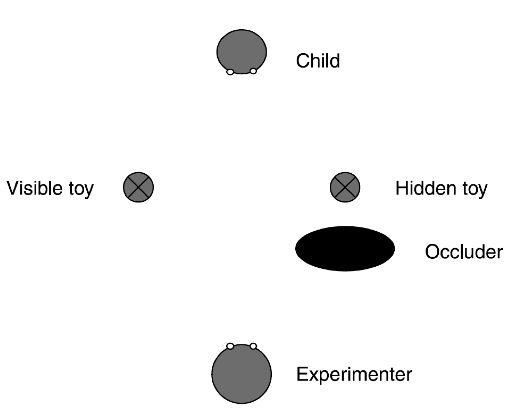
\includegraphics{figure_level_1_perspective_taking.png}
%\caption{
%\label{figure:level_1_perspective_taking}
%Experimental setup for Moll \& Tomasello’s 2006 experiment on level 1 perspective taking.  The experimenter was unable to see one of two objects clearly visible to the child.  When the experimenter asked `I cannot find it! … Can you give it to me?', two-year-olds reliably handed the hidden toy to the experimenter \citep[source: ][figure 1]{en_1202}.
%}
%\end{center}
%\end{figure}
%%
%The authors suggest that children of this age `knew what another person could and could not see when that differed from what they saw'.\footnote{
%	\citet[][p.\ 609]{en_1202}.  
%	Compare \citet[][p.\ 1210]{en_1550} who take subjects' success on a level 1 perspective taking task to show that they
%`could conceptually distinguish what they saw from what another person might see, [and] could think about what the other person saw rather than what they saw when asked to do so.'
%}
%An alternative possibility is that children were representing encountering rather than seeing.  Children may interpret the experimenter’s saying `Where is it? I cannot find it!'\ as expressing an inability to act.  If they also treat having encountered an object as a condition for acting on it, this would explain why they reliably handed the experimenter the object she was not encountering.\footnote{ 	Children in Moll and Tomasello’s experiment reliably work out that the experimenter is requesting something.  This suggests some understanding of pragmatics which could be taken as evidence of much richer theory of mind cognition.  The hypothesis about encountering is neutral on this issue.  Its purpose is only to show that success on these tasks may involve representing encounterings rather than seeings or perceptions.
%}



For another application of the second principle, consider Hare, Call and Tomasello’s finding that chimpanzees reliably adopt strategies which are appropriate given what dominant competitors know about the locations of food \citep[]{en_1545}.  In their `uninformed' condition, a subordinate chimpanzee observed a food item being hidden while a dominant competitor’s view was blocked (see Figure \vref{figure:hare_food_perception}).  In this condition subordinates chose to approach the food significantly more often than in a control condition where the dominant competitor saw the food being hidden.  This indicates that the subordinate chimpanzees were at least indirectly sensitive to facts about what the dominants had perceived.  Several explanations of this finding have already been suggested \citep[]{Call:2008di, en_1551, Suddendorf:2003co}.  A further possibility is that subordinate chimpanzees are aware that the dominant chimpanzee has not encountered the food and take encountering the food to be a condition for the dominant to act with the goal of recovering it.  That would enable them to predict that the subordinate will not be able to retrieve this food in the misinformed condition. 



\begin{figure}
\begin{center}
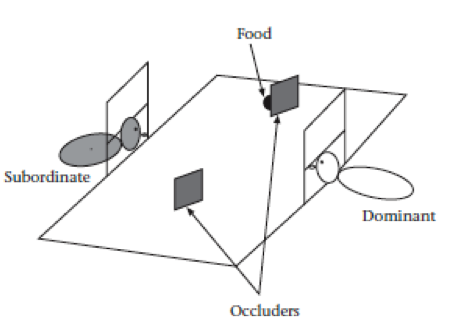
\includegraphics{figure_hare_food_perception.png}
\caption{
	\label{figure:hare_food_perception}
	A subordinate observes as food is placed.  The subordinate can also see the dominant.  There are three conditions: control—the dominant sees food being placed; `uninformed'—the dominant’s view is blocked while the food is placed; and `misinformed'—the dominant sees the food being placed then  has their view blocked while it is moved.
	 \citep[Source:][pp.\ 142, fig. 1]{en_1545}
}
\end{center}
\end{figure}


In short, 
one way to explain abilities to track others' perceptions  is to represent perceptions as such.
But another way to track perceptions is to represent encounterings and to suppose (as the second principle states) that goal-directed actions involving an object are only possible when the agent has encountered that object.


So far we have been taking for granted that representing encounterings is different from representing perceptions as such.
Why accept this claim? 
It is striking that philosophers have quite different views about what seeing involves—there are debates about whether it is possible to see things without seeing that something is the case \citep[e.g.][]{en_1671}, about whether and in what sense seeing is a representational notion \citep[]{en_1619, en_1705}, and about whether vision is intrinsically a source of knowledge \citep[]{en_1706}, for example.  
There is at least as much uncertainty concerning what might be involved in representing perceptions as such. 
So it is not possible for us to say with certainty what it is to represent perceptions as such.  
Even so, we can be sure that there are some differences between encountering and perception.
If perceptions are representations, then representing perceptions as such plausibly involves representing representations.
Since encounterings are relations not representations (by definition), representing encounterings will  differ from representing perceptions in that only the latter involves representing representations.
But, as mentioned, not everyone agrees that perceptions are representations.
We should therefore consider a bundle of features.
Perception constitutively involves appearances, modalities or the possibility of illusion or is constitutively linked to reasons, knowledge or informational states.
It is plausible that representing perceptions as such involves understanding something about some of these things.
Since encountering does not constitutively involve any of these (by definition), 
representing encounterings may differ from representing perceptions in that it does not require any kind of sensitivity to constitutive links with reasons, knowledge or informational states and nor does it require understanding  anything about appearances, modalities or the possibility of illusion.



\subsection{Third principle}

At this point we switch our attention from conditions on the \textit{occurrence} of goal-directed actions to conditions on their \textit{success}.  Such conditions are more stringent.  Where a goal specifies a particular object, it’s often not enough to have encountered it.  To succeed you must often also have encountered it \textit{in its current location} and to have done so \textit{on your most recent encounter}.  
(There are exceptions, of course.)

We can capture this condition and more by introducing a new notion, \textit{registration}.  Registration is a relation between an individual, an object and a location which will be implicitly defined by principles linking it to encountering and action.  (Where these principles conflict, principles mentioned later trump principles mentioned earlier.)  The first of these principles is that an individual registers an object at a location if she most recently encountered it at that location.  As is already clear from this principle, registration is like belief in that it has a correctness condition which may not obtain: a registration is correct when the object is in the location.   Since representing registration brings no benefit for Lucky independently of its connection to action, this principle cannot stand alone in our sequence; it is only the first half of the third principle.

The second half of the third principle states that correct registration is a condition of successful action.  More precisely, in order to successfully perform a goal-directed action with a goal that specifies a particular object, the agent must correctly register that object.%
\footnote{ 	
Some commentators suggested that this principle requires an ability to remember particular encounterings and their temporal order.  There is some evidence that some nonhumans possess this ability \citep[e.g.][]{en_1714, en_1715}, but our proposal does not depend on this.  To track another agent’s most recent encounter, it is not necessary to remember all encounters and their temporal order; forgetting all but the most recent will do.
}  
This principle can be applied in two directions.  In one direction, it licenses Lucky to predict that a competitor who does not have a correct registration of an object will not be successful in performing actions whose goals specify that object.  In the other direction, it allows Lucky, on the basis of observing a successful goal-directed action, to infer that the agent has correctly registered the location of an object.%
\footnote{ 	
The ‘other direction’ is required (in conjunction with the fifth principle, below) for explaining infants’ success on false belief tasks where information about another’s beliefs is provided not by what she sees but by what she does \citep[as in][]{en_1824}.
}
So the principle not only extends Lucky’s ability to predict actions but also her ability to detect what someone registers.  

The correctness of someone’s registrations can be manipulated in their absence by moving or destroying objects they have registered.  So with theory of mind cognition partially characterized by the third principle, Lucky can intentionally prevent others from stealing a food item they have already encountered simply by moving it in their absence.

For an application of this principle, consider Hare, Call and Tomasello’s (\citeyear[]{en_1545}) experiment again.  In a further condition, the `misinformed' condition, a subordinate observer watched as a dominant competitor saw food being hidden.  The subordinate continued to watch as the competitor’s view was blocked and the food moved.  In this case the competitor has encountered the food but does not correctly register it.  The subordinate observers went for the food more often in this condition than in a control condition where the dominant saw the food being moved.  This cannot be explained in terms of the third principle.  That principle involved taking encountering an object to be a condition on acting on it.  This condition is met: the competitor \textit{has} encountered the food.  To explain why the observer goes for the food that has been moved, we need to appeal to the third principle—to correct registration as a condition on success.  It is possible that the subordinate observer realized that the dominant competitor last encountered the food in a location other than its current location.  Suppose the observer also understood that correct registration is a condition on successful goal-directed action.  Then the observer could predict that the competitor would not succeed in retrieving the food.  This could explain why the observer approached the food in the `misinformed' condition.  

Another application of the third principle is to scrub-jays who strategically re-cache food depending on who saw what.  In one experiment, scrub-jays cached some food in the presence of Competitor A and then cached more food in the presence of Competitor B.  
Later they had an opportunity to recover food in the presence of Competitor A.  
The scrub-jays preferred to recover and re-cache food cached in the presence of Competitor A, leaving untouched food cached in the presence of the absent competitor \citep[][pp.\ 517-9]{en_1418}.  This strategy reduces the chances of Competitor A knowing where any of the scrub-jays’ food is.  What might explain this sensitivity to who saw what in choosing which food to recover?  Clayton and colleagues postulate a capacity to attribute knowledge or `informational states' \citep[]{en_1418}.  They are opposed by Penn and colleagues who postulate that scrub-jays are not ascribing knowledge but using rules such as `Try to re-cache food in a site different from the one where it was cached when the competitor was present' \citep[]{en_1417, Penn:2007ey}.  As an alternative to both proposals, the scrub-jays’ sensitivity could be explained in terms of registration.  Suppose scrub-jays understand that correct registration is a condition on successful goal-directed action.  Then they may be trying to prevent competitors from stealing their cached food by means of preventing them from correctly registering its location. As before, the motivation for our minimal theory of mind hypothesis is that it avoids the onerous information processing burden entailed by supposing that scrub-jays understand knowledge as such.    

A third application of this principle is to infant pointing.  Liszkowski and colleagues showed that 12- and 18-month-olds point in order to provide relevant information to adults about the locations of objects \citep[]{en_1093}.  In this experiment, infants watch as an adult uses an object in some task.  Then the adult appears to accidentally misplace it.  Later, when the adult visibly needs that object to complete the task again, infants reliably point to it.  Apparently infants point not in order to get the object or to share interest in it, but to enable the adult to complete a task.  The authors suggest that this could be explained either by supposing that infants understand what the adult does not know, or that they understand what the adult is not attending to \citep[][p.\ 185]{en_1093}.  As knowledge and attention are both complex psychological notions, these suggestions raise the hard question of what children might understand of them.  Registration suggests a third possible explanation.  Maybe these infants understand that correct registration is necessary for successful goal-directed action and that pointing is a way of generating correct registration.  (None of these explanations bear on what is perhaps most interesting about these findings, that infants care to inform others and do so spontaneously.  Minimal theory of mind as described here is at most a small part of a larger story.)





\section{***BIN***}


With these concepts in place, we can state the second principle: one can’t complete a goal-directed action on an object unless one is encountering it.  So for a goal-directed action to succeed it is not sufficient merely that the object is present; the agent must also be encountering the object.  This principle is not true but it is a useful heuristic.

The hypothesis that an individual tracks what others encounter is sufficient to explain success on some tests for level 1 perspective taking.  \citet[]{en_1550} asked children to hide objects from an experimenter.  The setup meant that the only hiding place left the objects in full view of the child herself.  Even the youngest children tested, two-and-a-half-year-olds, could do this reliably.  They were also able to say who could see an object in different conditions.  The researchers concluded that children can think about seeing:
%
\begin{quote}
`children could conceptually distinguish what they saw from what another person might see, [and] could think about what the other person saw rather than what they saw when asked to do so.'\footnote{
\citet[][p.\ 1210]{en_1550}.
Compare \citet[][p.\ 609]{en_1202} who take subjects' success on a level 1 perspective taking task to show that they
`knew what another person could and could not see when that differed from what they saw'.
}
\end{quote}
%
An alternative hypothesis consistent with these results is that children relied on knowledge of encountering rather than of seeing.  On this hypothesis, children interpreted the experimenter as requesting them to place the object where she would not be encountering it.  And they interpreted questions about who can see what in terms of who is encountering what.
Of course we  are not claiming that this is the best explanation of these findings.  
Our point is just that the ability to track perceptions measured by level 1 perspective taking tasks could involve representing encounterings only and need not involve representing perceptual states as such.
























\small
\bibliography{$HOME/endnote/phd_biblio_en_record_num_keys}

\end{document}